\documentclass{article}

\usepackage{lipsum}
\usepackage[margin=2cm, left=2cm, includefoot]{geometry}
\usepackage{graphicx}
\usepackage{float}
\usepackage{hyperref}

% Header and footer
\usepackage{fancyhdr}
\pagestyle{fancy}

\rhead{}
\lhead{}
\fancyfoot{}
\fancyfoot[R]{\thepage}
\renewcommand{\headrulewidth}{0pt}
\renewcommand{\footrulewidth}{0pt}
%

\begin{document}

\begin{titlepage}
	\begin{center}
		\line(1,0){300}\\
		[6mm]
		\huge{\bfseries PROJECT TENDER}\\
		[2mm]
		\line(1,0){200}\\
		[5mm]
		\large\textbf{PROJECT:}\\\textsc{Drone Mission Control - Agile}\\
		[3mm]
		\large\textbf{CLIENT:}\\\textsc{Retro Rabbit}\\
		[3mm]
		\large \textbf{TEAM:}\\\textsc{Funge}\\
		\line(1,0){350}\\
		[5mm]
		\large \textbf{Team Members:}\\
		[3mm]
		\large Matthew Botha\\
		\large Gian Paolo Buffo\\
		\large Matthias Harvey\\
        \large Dillon Heins\\[3mm]
		\begin{figure}[H]
			\centering
			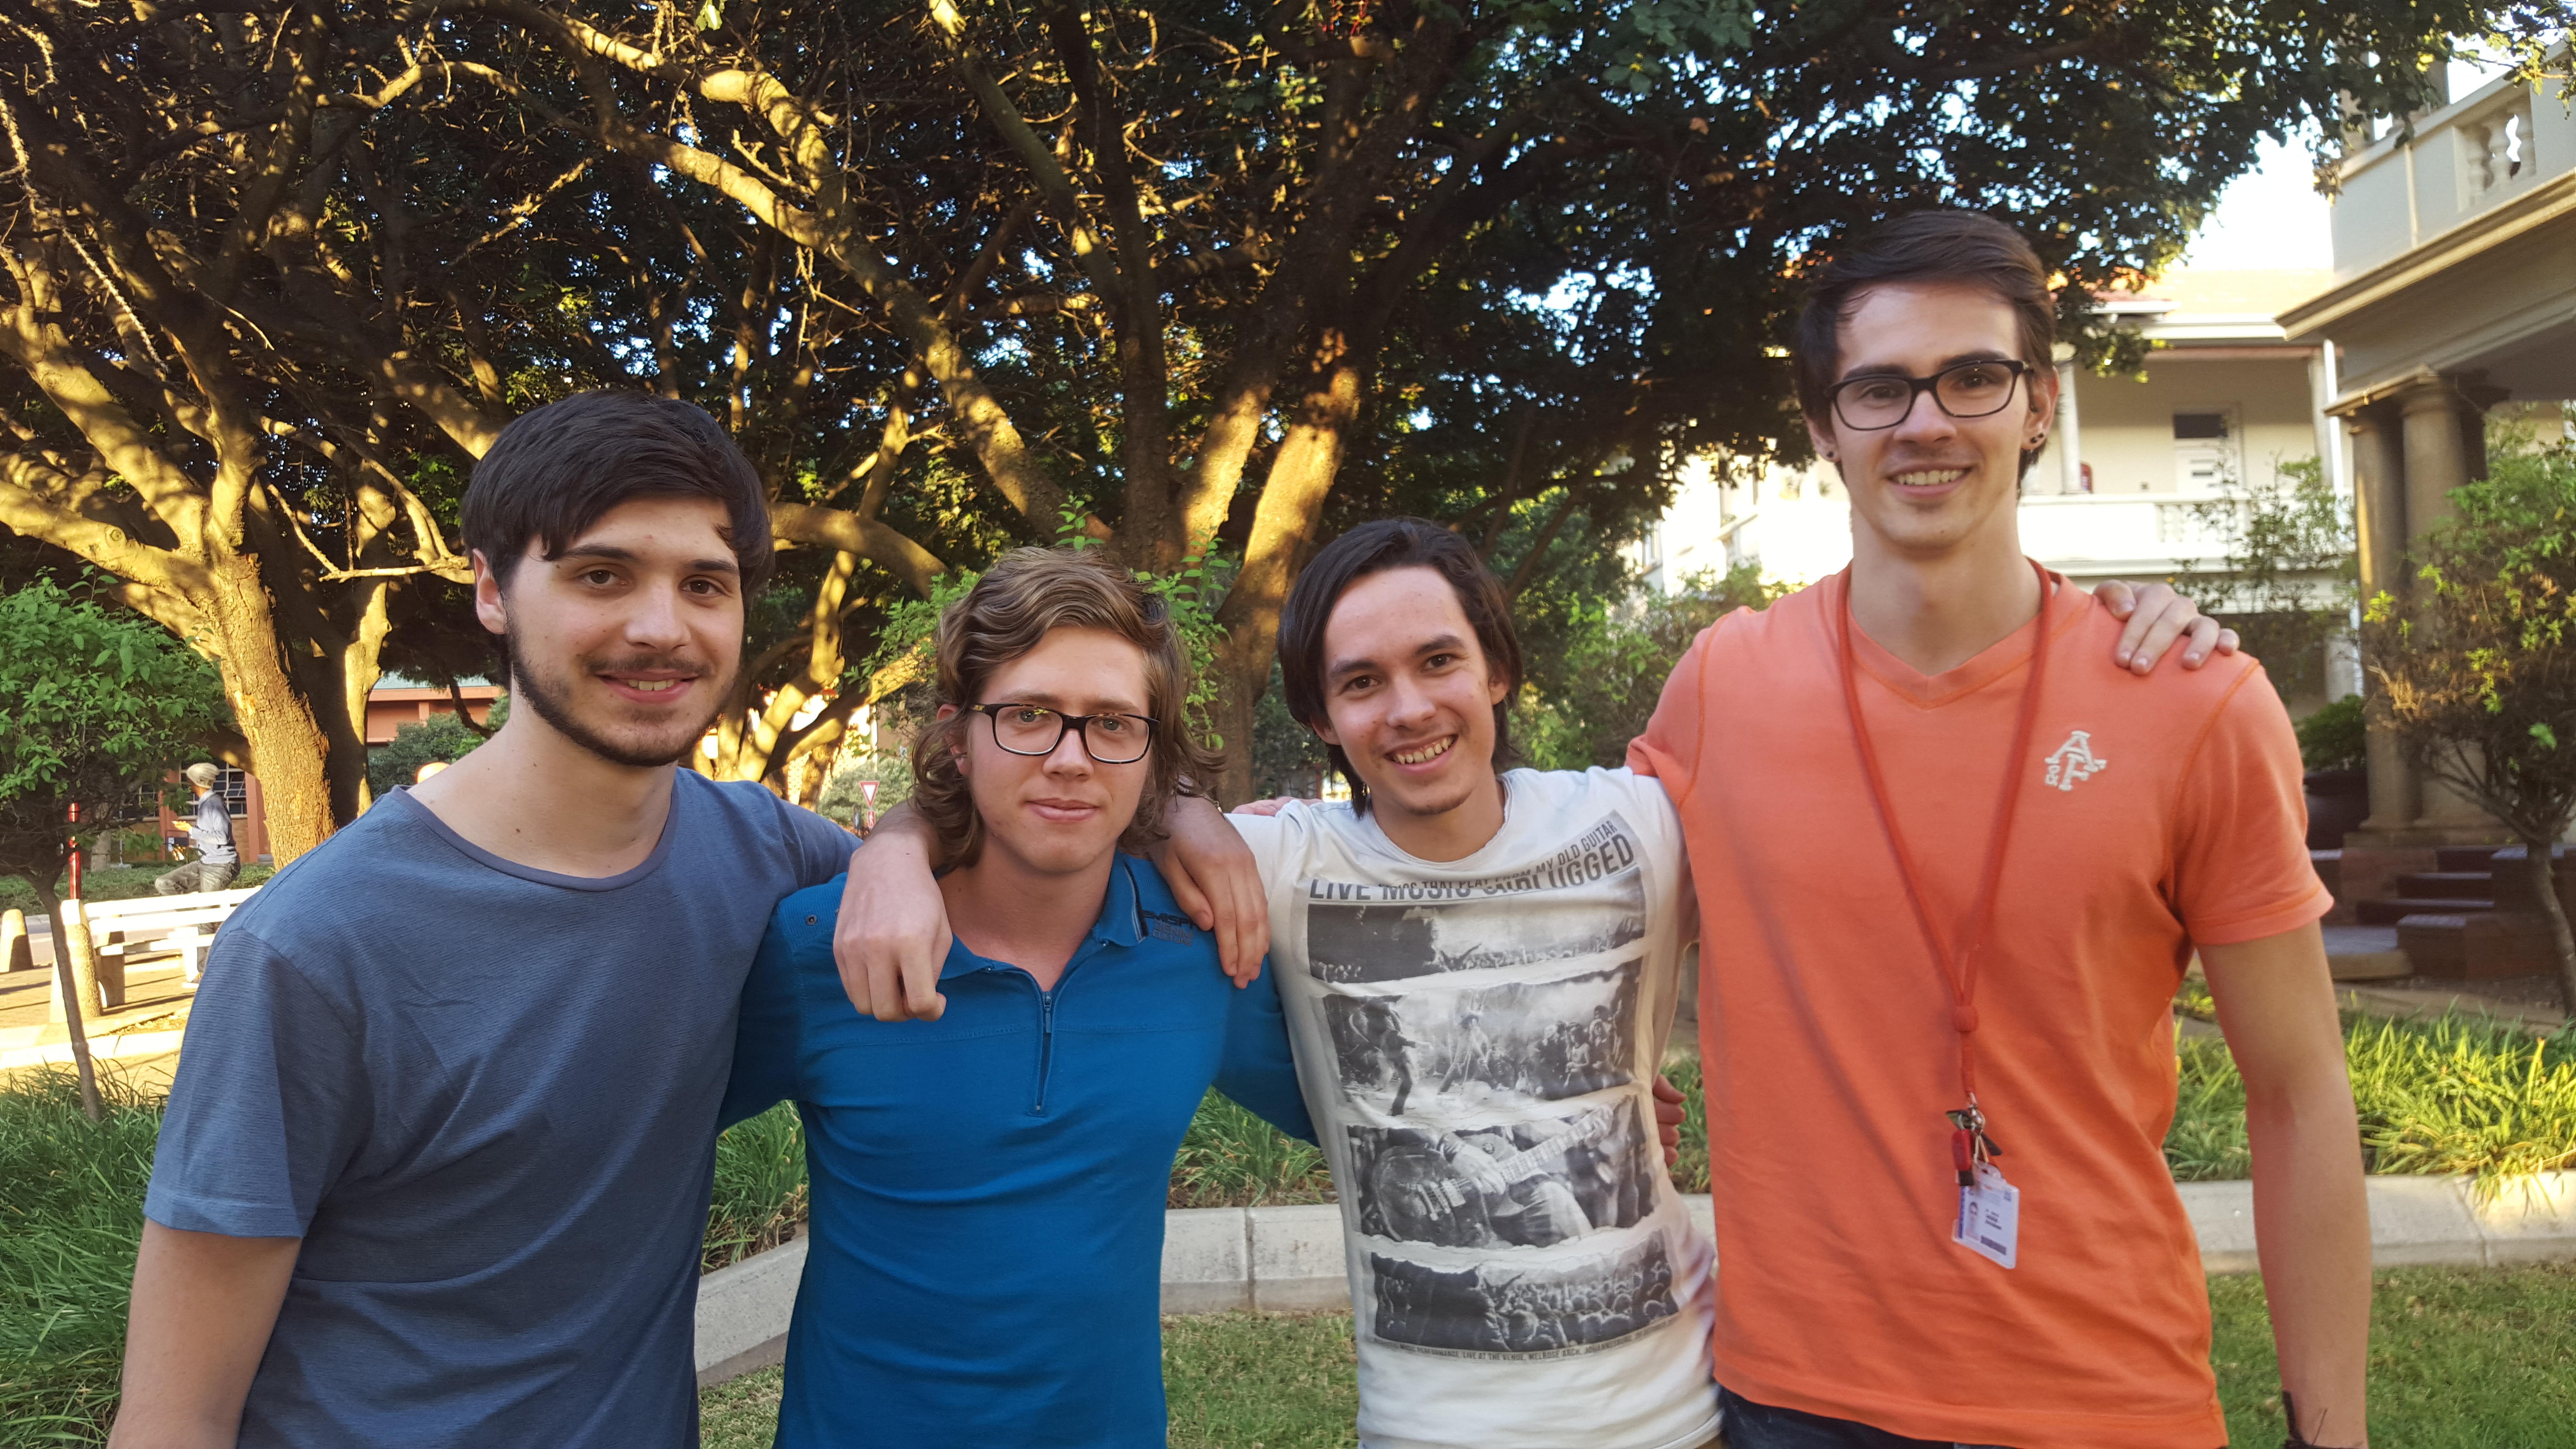
\includegraphics[width=0.8\textwidth]{../teamPhoto.jpg}
			\caption{Matthew Botha, Matthias Harvey, Gian Paolo Buffo, Dillon Heins}
		\end{figure}
    \end{center}

	\vspace{7mm}

    \begin{flushright}
        \textsc{\large Department of Computer Science\\
        University of Pretoria\\
        01 May 2016\\}
    \end{flushright}
\end{titlepage}

\section{The Team}
	\subsection{Matthew Botha}
		\subsubsection{Motivation for Choosing Project}
	
	\cleardoublepage	
			
	\subsection{Gian Paolo Buffo}
		\subsubsection{Motivation for Choosing Project}

	\cleardoublepage

	\subsection{Matthias Harvey}
		\subsubsection{Motivation for Choosing Project}
	
	\cleardoublepage
	
	\subsection{Dillon Heins}
		\subsubsection{Motivation for Choosing Project}

\cleardoublepage
    
\section{Project Execution}
	\subsection{Development Methodology}
		We intend to follow the Scrum approach to Agile software development throughout the course of project development. Agile itself is not a methodology and does not provide concrete steps which we would be able to follow. Hence we have opted to incorporate Scrum specific methods within the Agile movement. The reasons we have considered to use this methodology are as follows:
		\begin{itemize}
			\item The agile approach ensures that we as a team will be able to respond effectively and efficiently to unpredictability through incremental, iterative sprints
			\item These short sprints enable us to ensure that the product is kept in a potentially shippable state at all times
			\begin{itemize}
				\item This is effective as it ensures the product is always integrated and tested
				\item By having these short sprints of development it will enable us to periodically demonstrate our product to the client so that we are able to receive feedback, adapt to said feedback and plan accordingly for the next sprint
			\end{itemize}
			\item Scrum and agile work well together as Scrum is simple and flexible
			\item Scrum enables test-driven development
			\item Agile incorporates both the business and technical side and enables all involved with the project to engage and function together
			\begin{itemize}
				\item Scrum only has three roles: Product owner, Team, and Scrum Master
				\item These roles bode well to the nature of this project
			\end{itemize}
			\item To summarise: Scrum emphasises "empirical feedback, team self management, and striving to build properly tested product increments within short iterations"
			\begin{itemize}
				\item This ensures the continuous act of inspecting and adapting in order to deal with complexity and risk
				\item Our team is responsible for self management which enables us to function well without having to have continuous contact with our client
				\item Scrum decision making revolves around real-world situations and feedback rather than assumption
			\end{itemize}
		\end{itemize}
	\subsection{Methods of Informing Client}
	\subsection{Initial Ideas for Solving Technical Challenges}
	\subsection{Possible Technologies to Use for Project}
	\subsection{Final Deliverable}
\end{document}
